\usetikzlibrary{calc}


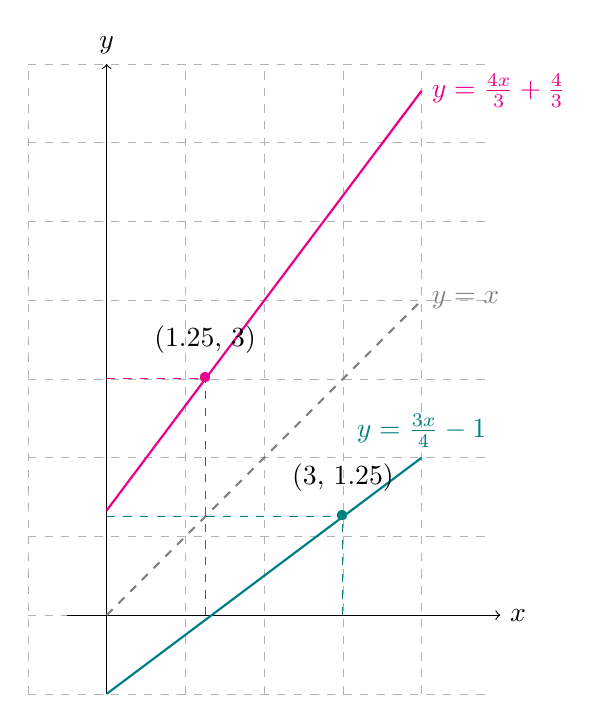
\begin{tikzpicture}
	\begin{scope}
\draw[help lines, color=gray!60, dashed] (-1,-1) grid (4.9,7);
\draw[->] (-0.5,0)--(5,0) node[right]{$x$};
\draw[->] (0,-1)--(0,7) node[above]{$y$};
\draw[thick,teal] (0,-1)--(4,2) node[above]{$y=\frac{3x}{4}-1$};
\draw[thick,magenta] (0,1.33)--(4,6.66) node[right]{$y= \frac{4x}{3}+ \frac{4}{3}$};
\draw[thick,gray,dashed] (0,0)--(4,4) node[right]{$y=x$};

\node [magenta, label={(1.25,$\ $3)}] at (1.25,3) {\textbullet};
\node [teal, label={(3,$\ $1.25)}] at (3, 1.25) {\textbullet};

\draw[thick,thin,teal,dashed] (3,0)--(3,1.25) node[right]{};
\draw[thick,thin,teal,dashed] (0,1.25)--(3,1.25) node[right]{};

\draw[thick,thin,magenta,dashed] (1.25,0)--(1.25,3) node[right]{};
\draw[thick,thin,magenta,dashed] (0,3)--(1.25,3) node[right]{};

	\end{scope}
\end{tikzpicture}
